\section{A weak Potts field as a tilt}\label{sec:frontier-modes}

In this section the start is uniform again. Give each visit to state $i$ the
extra weight $e^{h_i/N}$, for a fixed vector $h\in\mathbb R^d$. Over $N$ steps
these weights multiply to $e^{h\cdot n/N}$, a factor of order $1$, which is the
scale of the constants $a_k$. So the field can reorder the faces. We study the
\emph{tilted occupation law}
\begin{equation}\label{eq:weakfield-law}
 \widetilde P_{N,h}(n)=
 \frac{e^{h\cdot n/N}P_N(n)}
 {\sum_{m_1+\cdots+m_d=N}e^{h\cdot m/N}P_N(m)}.
\end{equation}
We use the window coordinate $T=L-\frac12\log L+t$. The normalizing sum cancels
whenever we compare two bins. A modal phase is the support of the global
modes, which need not be the face with most of the mass.

\begin{proposition}[the field is a tilt]\label{prop:field-tilt}
Let $\Lambda_N(h)=\log\E\exp\langle h,K_N/N\rangle$.
\begin{enumerate}[(1)]
\item $\widetilde P_{N,h}(n)=\exp\bigl(\langle h,n/N\rangle-\Lambda_N(h)\bigr)P_N(n)$.
So $\widetilde P_{N,h}$ is the exponential tilt of the law of the occupation
rate $K_N/N$ by the linear function $\langle h,\cdot\rangle$.
\item It is also the law of the counts when the law of the path is tilted by
$\exp(\sum_{s=1}^Nh_{X_s}/N)$. This is the Potts chain with free boundaries,
coupling $p/r$ per equal neighbor pair and field $h/N$ at each site.
\item If $T\to\infty$, then $\Lambda_N(h)\to\bar h=\frac1d\sum_ih_i$.
\end{enumerate}
\end{proposition}

\begin{proof}
Part (1) is~\eqref{eq:weakfield-law} with its denominator written as
$e^{\Lambda_N(h)}$. For (2), a word $x_1\cdots x_N$ has probability
$\frac1dr^{N-1}(p/r)^{\sum_{s<N}\delta(x_s,x_{s+1})}$, and
$\sum_sh_{x_s}=\langle h,n\rangle$ depends on the word only through its counts
$n$. So tilting the words and then counting gives (1).

For (3), the chain is stationary with transition matrix
$\sigma I+(1-\sigma)\frac1dJ$, whose $m$-th power is
$\sigma^mI+(1-\sigma^m)\frac1dJ$. So $\E K_{N,a}=N/d$, and the indicators of
state $a$ at times $s$ and $s+m$ have covariance $\sigma^m(\frac1d-\frac1{d^2})$.
Summing over the two times gives, for $p<1$,
\[
 \Var K_{N,a}=\Bigl(\frac1d-\frac1{d^2}\Bigr)
 \Bigl(N\,\frac{1+\sigma}{1-\sigma}-\frac{2\sigma(1-\sigma^N)}{(1-\sigma)^2}\Bigr).
\]
We bound this in two cases. Note that $1-\sigma=dr$. If $1/d\le p<1$, then
$0\le\sigma<1$, the second term in the bracket is not positive, and
$\Var(K_{N,a}/N)\le2/(d^2T)$. If $p<1/d$, then $-1\le\sigma<0$, the bracket is
at most $N+4$, and $T\le N$, so $\Var(K_{N,a}/N)\le5/T$. In both cases
$K_N/N$ tends to the uniform vector in probability as $T\to\infty$. Since
$\exp\langle h,K_N/N\rangle$ is bounded, bounded convergence gives the limit.
\end{proof}

By (1), $|\log\widetilde P_{N,h}(n)-\log P_N(n)|\le2\max_i|h_i|$ for every $n$.
This is of the order of the constants $a_k$, but invisible at first order, so
a field of total size $o(\log N)$ does not change the exponents of
Theorem~\ref{thm:simplex-window}(ii). For a support $S$ with $|S|\ge2$ put
$\bar h_S=\frac1{|S|}\sum_{i\in S}h_i$.

\begin{theorem}[weak-field modal phase diagram]\label{thm:weakfield-phases}
Put $T=L-\frac12\log L+t$ and define the face scores
\[
 \ell_S(t,h)=
 \begin{cases}
 h_i,& S=\{i\},\\
 (|S|-1)(t-a_{|S|})+\bar h_S,& |S|\ge2.
 \end{cases}
\]
The largest bin weight, taken relative to the untilted vertex and before the
normalization in~\eqref{eq:weakfield-law}, satisfies, uniformly for $(t,h)$ in
compact sets,
\begin{equation}\label{eq:weakfield-maximum}
 \log\max_n\left\{e^{h\cdot n/N}\frac{P_N(n)}{V_N}\right\}
 \longrightarrow \max_{\varnothing\ne S\subseteq\{1,\ldots,d\}}
 \ell_S(t,h).
\end{equation}
For fixed $(t,h)$ and all large $N$, every global mode has a support that
maximizes the limiting score. If the maximizing support is unique, all global
modes have exactly that support. On a selected support $S$ with $|S|\ge2$,
their locations satisfy
\[
 \max_{i\in S}\left|\frac{n_i}{N}-\frac1{|S|}\right|=o((\log N)^{-1/2}).
\]
This does not identify the maximizing vectors exactly, and equal limiting
scores do not imply that both supports hold modes at finite $N$.

If the fields are sorted as $h_1\ge\cdots\ge h_d$, the maximum of the scores is
the upper envelope of the $d$ lines
\begin{equation}\label{eq:weakfield-lines}
 \ell_1(t)=h_1,\qquad
 \ell_k(t)=(k-1)(t-a_k)+\frac1k\sum_{i=1}^k h_i,
 \quad 2\le k\le d.
\end{equation}
Away from ties, the winning support size is nondecreasing in $t$. If the fields
are strictly ordered, the winning supports are the nested sets
$\{1,\ldots,k\}$. Every support size $k\in\{2,\ldots,d-1\}$ is the unique
winning size on an open interval of $t$ for suitable fixed fields. So
proper-face phases persist under a field of order $1/N$ per step.
\end{theorem}

So the field shifts the line of each face by the field averaged over the face.
Indeed, on a support $S$ the ratio of a bin to a vertex has a Gaussian profile of
width $1/\sqrt L$ around the center of the face (Lemma~\ref{lem:confinement}),
where the tilt is $e^{\bar h_S+o(1)}$. The proof is in
Appendix~\ref{app:start-field}.

\begin{example}[a persistent triangular edge phase]\label{ex:weakfield-triangle}
For $d=3$ and $h=(0,0,-H)$ the three competing scores are $0$, $t-a_2$ and
$2(t-a_3)-H/3$. If $H>6(a_2-a_3)$, the edge $\{1,2\}$ wins strictly for
\[
 a_2<t<H/3+2a_3-a_2,
\]
and for every fixed $t$ in this interval all global modes of the tilted law lie
on that edge for large $N$. Without a field no proper face holds a mode in the
window (Corollary~\ref{cor:simplex-modes}).
\end{example}


One field can make every support size win in turn, from one state to all $d$.

\begin{corollary}[one field realizes the full face hierarchy]
\label{cor:weakfield-full-hierarchy}
Fix $d\ge2$ and $H>3/4$, and let $h_i=-H(i-1)^2$ for $1\le i\le d$. In
particular $h_i=-(i-1)^2$ works in every fixed dimension. Put
\[
 c_k=(k+\tfrac12)\log k-\frac{k-1}{2}\log(4\pi),\qquad
 t_k=c_k-c_{k+1}+\frac{H(4k-1)}6\quad(1\le k<d),
\]
and $t_0=-\infty$, $t_d=+\infty$. Then $t_1<\cdots<t_{d-1}$, and for every
$k\in\{1,\ldots,d\}$ the support $\{1,\ldots,k\}$ is the unique winning support
on the nonempty interval $t_{k-1}<t<t_k$. So for each fixed $t$ in this
interval and all large $N$, every global mode of the tilted law has exactly
those $k$ positive coordinates.
\end{corollary}

Here $c_1=0$ and $c_k=\log D_k$ for $k\ge2$. Figure~\ref{fig:phases} shows the
lines for $d=5$, and the proof is in Appendix~\ref{app:start-field}.

\begin{figure}[t]
\centering
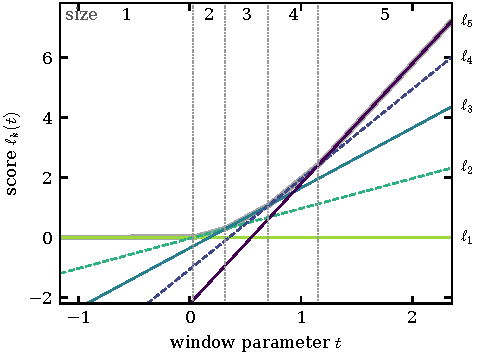
\includegraphics{figures/phases}
\caption{The lines~\eqref{eq:weakfield-lines} for $d=5$ and $h_i=-(i-1)^2$. The
gray band is their upper envelope. The dotted lines are $t_1<\cdots<t_4$, and
the number at the top of each interval is the size $k$ of the winning support
$\{1,\ldots,k\}$.}
\label{fig:phases}
\end{figure}

